% Created 2019-04-08 Mon 16:57
\documentclass[presentation]{beamer}
\usepackage[utf8]{inputenc}
\usepackage[T1]{fontenc}
\usepackage{fixltx2e}
\usepackage{graphicx}
\usepackage{longtable}
\usepackage{float}
\usepackage{wrapfig}
\usepackage{rotating}
\usepackage[normalem]{ulem}
\usepackage{amsmath}
\usepackage{textcomp}
\usepackage{marvosym}
\usepackage{wasysym}
\usepackage{amssymb}
\usepackage{hyperref}
\tolerance=1000
\usetheme{default}
\author{Jonatan Ahumada Fernández}
\date{\today}
\title{Fedora}
\logo{
\includegraphics[height=1.5cm]{logo}}
\hypersetup{
  pdfkeywords={},
  pdfsubject={},
  pdfcreator={Emacs 25.3.1 (Org mode 8.2.10)}}
\begin{document}

\maketitle
\begin{frame}{Outline}
\tableofcontents
\end{frame}


\begin{frame}[label=sec-1]{PREAMBULO (corto)}
\begin{quote}
A Linux distribution consists of the components needed to create a working Linux system and the procedures needed to get those components installed and running.
 Technically, Linux is really just what is referred to as the kernel.
 Before the kernel can be useful, you must have other software such as basic commands (GNU utilities),
 services you want to offer (such as remote login or web servers), and possibly a desktop interface and graphical applications.
 Then, you must be able to gather all that together and install it on your computer’s hard disk.
\end{quote}
\end{frame}
\begin{frame}[label=sec-2]{HISTORIA \& EVOLUCION}
\begin{block}{Entra en escena Red Hat}
\begin{quote}
Before long, many other Linux distributions were created.
 Some Linux distributions were created to meet special needs, such as KNOPPIX (a live CD Linux), Gentoo (a cool customizable Linux), and Mandrake (later called Mandriva, which was one of several desktop Linux distributions).
 But two major distributions rose to become the foundation for many other distributions: Red Hat Linux and Debian.
\end{quote}
\end{block}
\end{frame}

\begin{frame}[label=sec-3]{Nace Fedora}
\begin{quote}
 Red Hat, Inc. gave away the source code, as well as the compiled,
For years, Red Hat Linux was the preferred Linux distribution for both Linux professionals and enthusiasts.
ready-to-run versions of Red Hat Linux (referred to as the binaries).
 But as the needs of their Linux community users and big-ticket customers began to move further apart,
 Red Hat abandoned Red Hat Linux and began developing two operating systems instead: Red Hat Enterprise Linux and Fedora. (Linux Bible, Cristopher Negus)
\end{quote}
\end{frame}
\begin{frame}[label=sec-4]{Tecnología de punta}
\begin{quote}
Using Fedora
While RHEL is the commercial, stable, supported Linux distribution, Fedora is the free, cutting-edge Linux distribution that is sponsored by Red Hat, Inc.
Fedora is the Linux system Red Hat uses to engage the Linux development community and encourage those who want a free Linux for personal use.
Fedora includes more than 16,000 software packages, many of which keep up with the latest available open source technology.
 As a user, you can try the latest Linux desktop, server, and administrative interfaces in Fedora for free. As a software developer, you can create and test your applications using the latest Linux kernel and development tools.
Because the focus of Fedora is on the latest technology, it focuses less on stability. (Linux Bible, Cristopher Negus)
\end{quote}
\end{frame}


\begin{frame}[label=sec-5]{Razones para usar Fedora}
\begin{itemize}
\item Cambió el paradigma de archivos comprimidos a archivos con metadatos (local RPM database, removerlo, atualizarlo, etc)
\item Intalación simple, al estilo de los "wizard", en muchos casos los valores predefinidos bastaban.
\item Administración gráfica:se podía utilizar sin necesidad de hacer comandos.
\item Incluye funcionalidad de Red Hat de tipo empresarial (por ejemplo, facilidad para montar una base de datos para una red interna).
\end{itemize}

\begin{block}{Ejemplos de funcionalidades empresariales}
\begin{itemize}
\item Kickstart files
\item PXE boot
\item Satellite server (Spacewalk)
\end{itemize}
\end{block}
\end{frame}

\begin{frame}[label=sec-6]{Historia de las versiones}
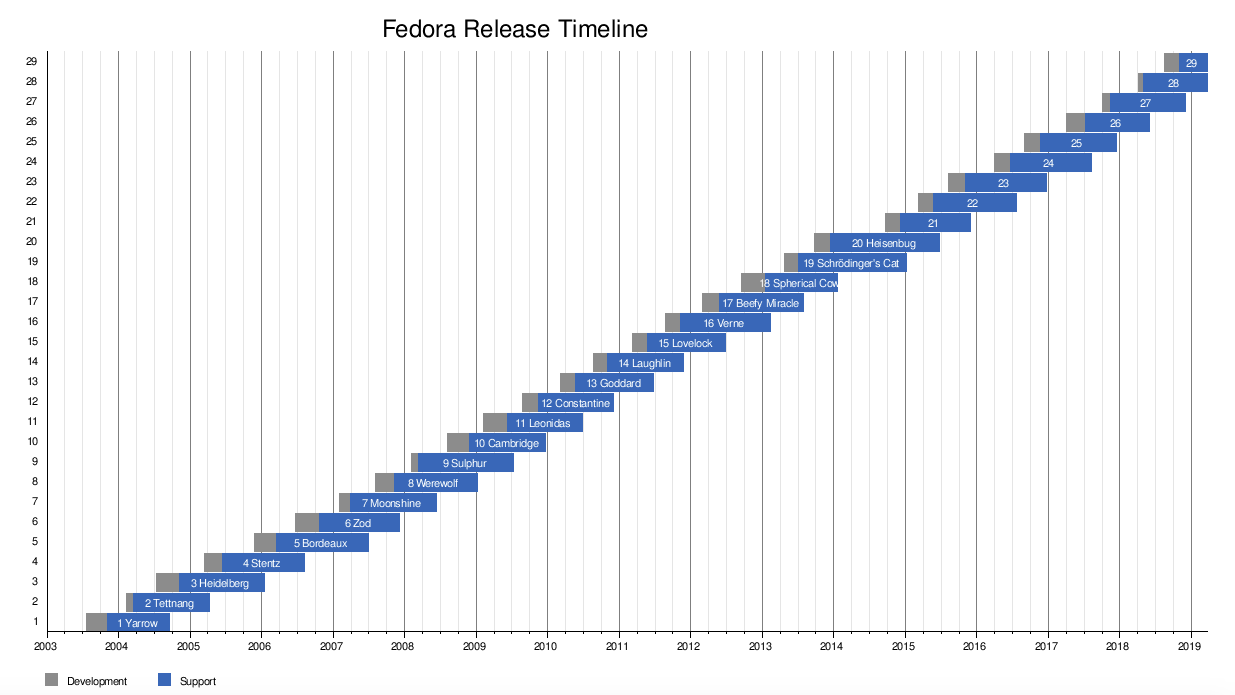
\includegraphics[width=.9\linewidth]{./timeline.png}
(Tomado de: www.fedoraproject.org)
\end{frame}

\begin{frame}[label=sec-7]{FABRICANTE S.O}
\url{https://docs.fedoraproject.org/en-US/project/}
\begin{quote}
The Fedora Project is not a separate and distinct legal entity.
 Red Hat, the primary sponsor of the Fedora Project, is actively involved in legal matters relating to Fedora, along with other Fedora participants.
 For example, Red Hat lawyers assist Fedora Project contributors in issues pertaining to free and open source software licensing, trademarks and patents.
 Refer to the Legal page for more information. (Tomado de: www.fedoraproject.org)
\end{quote}

\begin{block}{Jugadores Principales}
\begin{itemize}
\item Red Hat Inc.
\item Fedora Council
\item Fedora Engeneering and Steering Committee (FESCo)
\end{itemize}
\end{block}
\end{frame}
\begin{frame}[label=sec-8]{Organización}
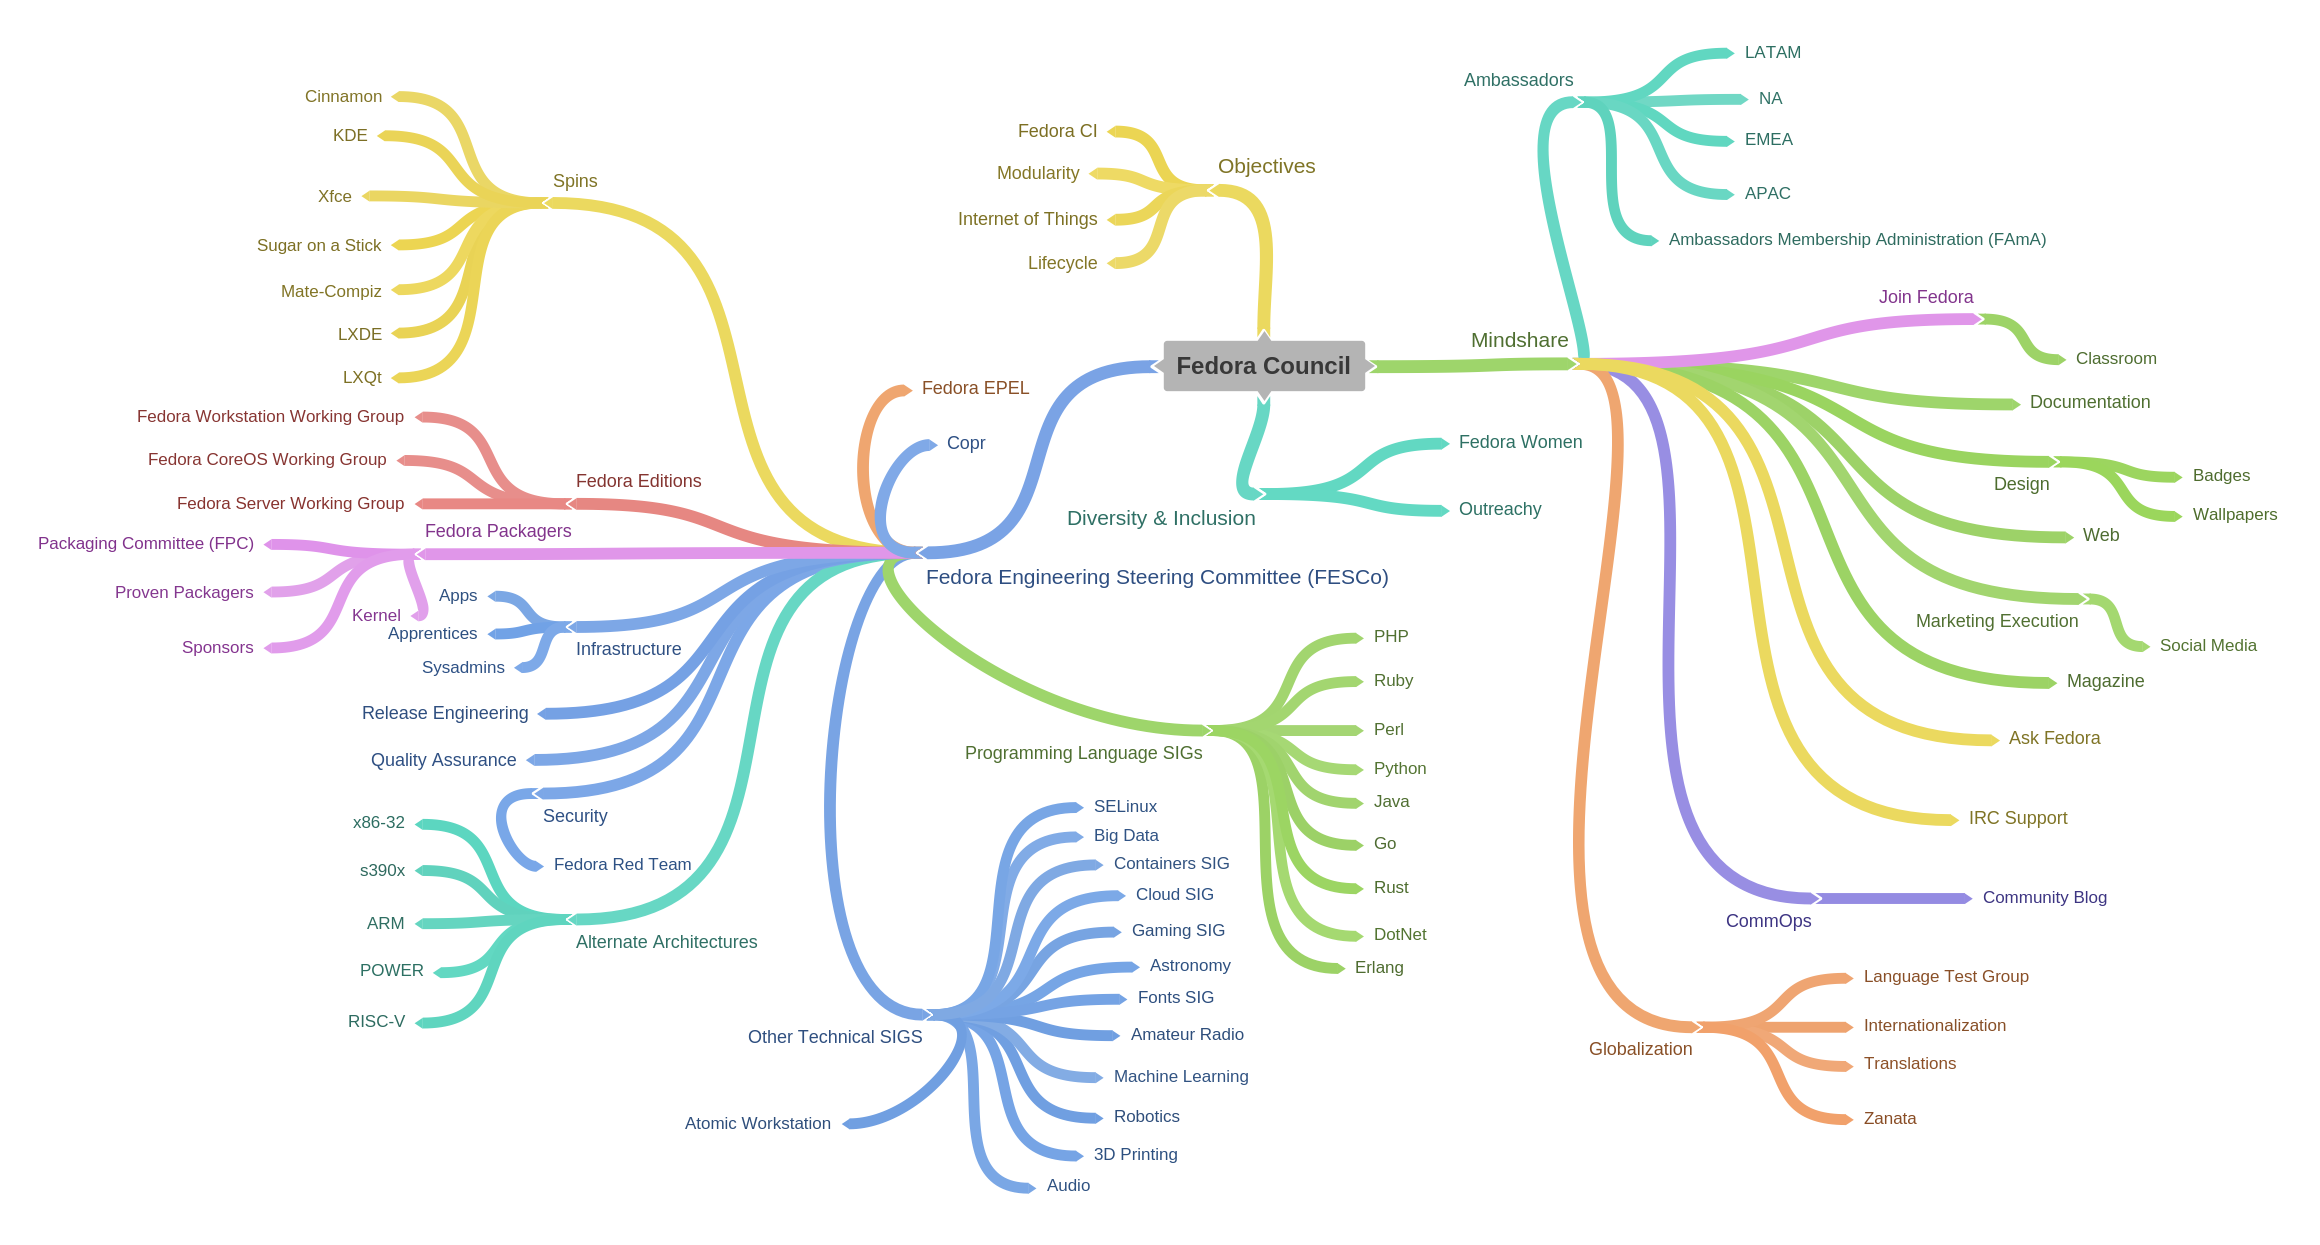
\includegraphics[width=.9\linewidth]{./orgchart.png}
(Tomado de: www.fedoraproject.org)
\end{frame}

\begin{frame}[label=sec-9]{CARACTERISTICAS}
\begin{itemize}
\item Freedom
\begin{itemize}
\item Repositorios principales son Open Source
\item Licencias \url{https://fedoraproject.org/wiki/Licensing:Main#Good_Licenses}
\end{itemize}
\item Friends
\begin{itemize}
\item Comunidad robusta
\item Ayuda técnica
\item Interfáz pulida
\item Instalación fácil
\item Documentación
\end{itemize}
\item Features 
\begin{itemize}
\item Workstation
\item Server
\item Atomic
\item Y muchos spins\ldots{}
\end{itemize}

\item First 
\begin{itemize}
\item Innovación
\item Rolling Release
\end{itemize}
\end{itemize}

Estas han hecho que Fedora se conozca como "para desarrolladores".
\end{frame}

\begin{frame}[label=sec-10]{Una nota sobre "Features"}
\begin{itemize}
\item Versiones
\begin{itemize}
\item Workstation
\begin{itemize}
\item Silverblue
\end{itemize}
\item Server
\item Atomic
\end{itemize}
\item Ediciones
\begin{itemize}
\item Plasma
\item XDE
\item XFCE
\item LXQT
\item Cinammon
\item Mate etc.
\end{itemize}
\item Fedora Labs 
\begin{itemize}
\item Astronomy
\item Design Suit
\item Scientific
\item JAM
\end{itemize}
\item Rawhhide
\end{itemize}
\end{frame}


\begin{frame}[label=sec-11]{APLICACIONES}
\end{frame}
\begin{frame}[label=sec-12]{Instalación Base (GNOME)}
\begin{itemize}
\item Suite Libre Office
\item Mapas
\item Rythmbox
\item Cajas(Boxes)
\item Calculadora
\item Fotos
\item Cheese
\item Calendario
\item Contactos
\end{itemize}
\end{frame}
\begin{frame}[label=sec-13]{Aplicaciones CLI}
\begin{itemize}
\item Compatibilidad con Docker incorporada
\item GNOME Boxes
\item COPR
\item Modularity
\item Git
\item Dev Assistant
\item Ver más en : \url{https://developer.fedoraproject.org/}
\end{itemize}
\end{frame}
\begin{frame}[label=sec-14]{Ejemplo de Modularidad}
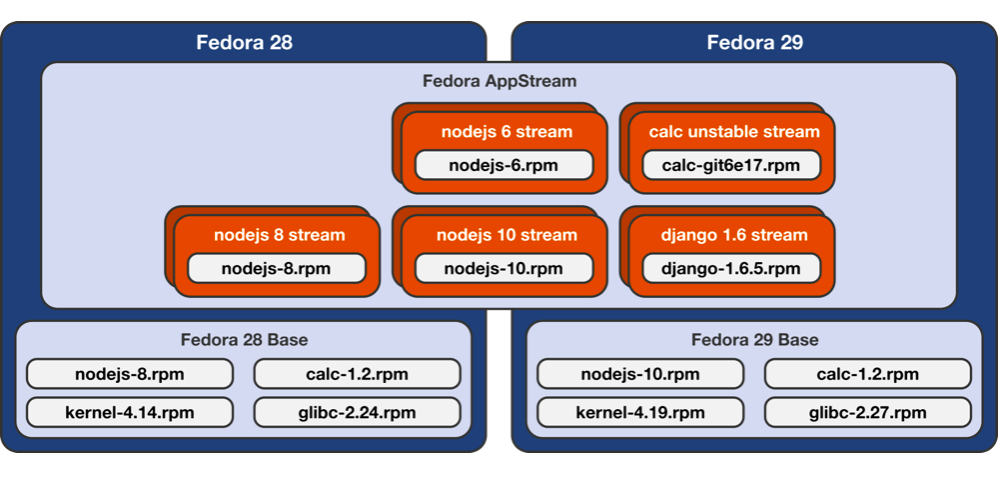
\includegraphics[width=.9\linewidth]{./modularity.png}
\end{frame}


\begin{frame}[fragile,label=sec-15]{Prueba para montar servidor Apache}
 \begin{verbatim}
sudo dnf install httpd
sudo systemctl start httpd.service
// verificar http//:localhost
\end{verbatim}
\end{frame}
\begin{frame}[fragile,label=sec-16]{Iniciar proyecto con dev assistant}
 \begin{verbatim}
da create java maven --name MyJavaApp --github
\end{verbatim}

Al parecer este paquete ya no está en uso, pero inició solo como un paquete de Fedora, luego 
se generalizó a un paquete de Python que se puede instalar con
\begin{quote}
pip3 install devassistant --user
\end{quote}
\end{frame}

\begin{frame}[fragile,label=sec-17]{Iniciar Proyecto con Docker}
 \begin{verbatim}
da create python django --name MyAppName --docker
\end{verbatim}
\end{frame}

\begin{frame}[label=sec-18]{HERRAMIENTAS DE SUPERVISION DE RENDIMIENTO}
\begin{block}{CLI}
\begin{itemize}
\item ps
\item top
\item jobs (foreground/background)
\item kill
\item killall
\item nice
\item renice
\end{itemize}
\end{block}

\begin{block}{GUI}
\begin{itemize}
\item Son dependientes del entorno de escritorio
\item En GNOME está monitor
\item hay guis simplificadas (system-config-[expresion]) dentro de los repositorios de Fedora, ejemplo: system-config-language
\end{itemize}
\end{block}
\end{frame}



\begin{frame}[label=sec-19]{REQUERIMIENTOS}
\begin{itemize}
\item Mínimos

\item 1GHZ  or faster processor
\item 1GB System Memory
\item 10GB unallocated drive space
\end{itemize}


\begin{itemize}
\item Recomendados

\item 2GHz dual core processor
\item 4GB System Memory
\item 20GB unallocated drive space
\end{itemize}
\end{frame}



\begin{frame}[label=sec-20]{VENTAJAS \& DESVENTAJAS}
\begin{block}{Principales}
Pros
\begin{itemize}
\item muy fácil de instalar
\item muchísimo soporte
\item Apariencia "comercial"
\item cubre muchos casos de uso (programadores, músicos, etc)
\item Une lo mejor de los dos mundos (OpenSource con enfoque empresarial)
\end{itemize}


Cons
\begin{itemize}
\item no soporta drivers propietarios (toca usar third party software)
\item es gigante: 10gb el iso
\item Excesiva funcionalidad
\item hay problemas con actualización de un lanzamiento a otro
\item puede ser lento (la VM a veces se queda con más de las especifiaciones mínimas)
\end{itemize}
\end{block}
\end{frame}

\begin{frame}[label=sec-21]{Debian}
\begin{center}
\begin{tabular}{ll}
Fedora & Debian\\
\hline
ciclo de vida corto & ciclo de vida largo\\
OpenSource + RedHat & Meritocracia\\
RPM & DEB\\
Anaconda & Documentacion, aunque ya no\\
Configuracion robusta & Configuración manual\\
Innovacion & Estabilidad\\
Funcionalidad & Seguridad\\
\end{tabular}
\end{center}
\end{frame}




\begin{frame}[label=sec-22]{Windows}
\begin{center}
\begin{tabular}{ll}
Fedora & Windows\\
\hline
ciclo de vida corto & Ciclo de vida largo\\
OpenSource + RedHat & Orientado a empresas\\
RPM & trabaja con .exe\\
Anaconda & El de windows, similares\\
Configuracion robusta & Todo "funciona"\\
Innovacion & Extensión (hardware y drivers funcionan)\\
Funcionalidad & $$$$\\
\end{tabular}
\end{center}
\end{frame}


\begin{frame}[label=sec-23]{Arch}
\begin{center}
\begin{tabular}{ll}
Fedora & Arch\\
\hline
Lanzamientos  rapidos & "frozen" release\\
OpenSource + RedHat & Meritocracia\\
RPM-Yum,-DNF & Pacman (una sola herramienta)\\
Anaconda & La 'mejor' docuemntación\\
Configuracion robusta & Recae completamente en el usuario\\
Innovacion & Customizacion\\
Funcionalidad & Simplicidad\\
Inestable & Más inestable (tú eres responsable)\\
 & Es "la que sirve para aprender"\\
\end{tabular}
\end{center}
\end{frame}
% Emacs 25.3.1 (Org mode 8.2.10)
\end{document}
